\subsection{Resultados del algoritmo secuencial}


\subsubsection{Optimización del código}

Para el algoritmo secuencial se uso una optimización por compilador con las banderas \texttt{-O3 -Wall -march=native -funroll-loops -flto -ffast-math -fomit-frame-pointer}, lo que permitió mejorar el rendimiento del código sin modificar su estructura. Esta optimización se tradujo en una reducción significativa del tiempo de ejecución, especialmente para matrices de mayor tamaño, al permitir al compilador aplicar técnicas avanzadas de optimización como la vectorización y el desenrollado de bucles.

El signigicado de cada bandera es el siguiente:
\begin{itemize}
   \item \textbf{-O3:} Esta bandera habilita un nivel de optimización agresivo, permitiendo al compilador aplicar una amplia gama de técnicas para mejorar el rendimiento del código.
   \item \textbf{-Wall:} Activa la mayoría de las advertencias del compilador, lo que ayuda a identificar posibles problemas en el código que podrían afectar su rendimiento o funcionalidad.
   \item \textbf{-march=native:} Permite al compilador generar código optimizado para la arquitectura específica del procesador en el que se está compilando, aprovechando las características y capacidades de hardware disponibles.
   \item \textbf{-funroll-loops:} Habilita el desenrollado de bucles, lo que puede mejorar el rendimiento al reducir la sobrecarga de control de bucle y aumentar la paralelización de las instrucciones.
   \item \textbf{-flto:} Habilita la optimización a nivel de enlace, lo que permite al compilador realizar optimizaciones globales en todo el programa, incluso entre diferentes archivos de código fuente.
   \item \textbf{-ffast-math:} Permite al compilador realizar optimizaciones agresivas en operaciones matemáticas, lo que puede mejorar el rendimiento a costa de la precisión en algunos casos como la evaluación de funciones trigonométricas.
   \item \textbf{-fomit-frame-pointer:} Indica al compilador que no utilice un puntero de marco para las funciones, es decir, que no cree un marco de pila para cada función, lo que puede mejorar el rendimiento al reducir la cantidad de instrucciones necesarias para gestionar la pila de llamadas.
\end{itemize}

\newpage

Estos fueron los tiempos de ejecución obtenidos para el algoritmo secuencial optimizado:
   \begin{figure}[H]
      \centering
      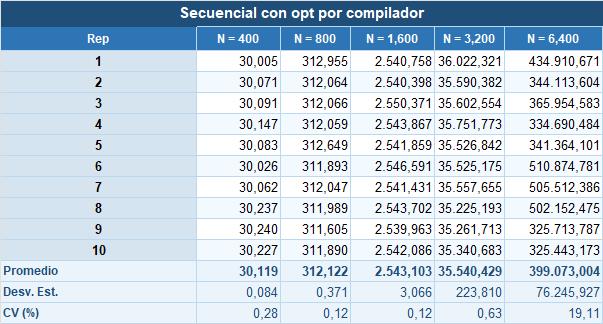
\includegraphics[width=1\textwidth]{images/tables/sec_opt.png}
      \caption{Tiempos de ejecución del algoritmo secuencial para diferentes tamaños de matriz.}
      \label{fig:secuencial}
   \end{figure}
   